\section{Discussion and extensions}\label{sec:discussion}
\subsection{What the Swedish replication adds}

The Swedish results qualify a simple disappearing-effect narrative in three ways. First, the later-decade addition return is positive under several separately reported specifications. Second, the early-to-late decline is not a steady progression, and its magnitude depends on which part of the reconstitution episode is measured. Third, smaller implementation-window returns coexist with more concentrated trading immediately before effectiveness. The contribution is the joint evidence on returns, measurement and trading in a scheduled-review setting, rather than a claim that a single coefficient overturns the US findings.

This distinction also clarifies the comparison with Greenwood and Sammon. Their question links a changing price response to index demand and market capacity to absorb it. The Swedish data allow a related investigation, but neither the country nor the period is held constant against the US. The shortened announcement lead time is an additional institutional feature that must enter the interpretation of the Swedish full-window series. A return over a shorter implementation interval is not automatically a weaker response to the announcement itself.

The fixed-window calculation makes this point concrete. The latest-minus-earliest addition contrast is approximately -7.03 percentage points for the full episode and +0.62 points for the common first seven daily returns. The remaining interval contributes -7.64 points to the difference. The initial seven-day contrast is imprecise, with a 95\% analytical interval of [-1.80, 3.03]. We therefore do not establish equal announcement responses or a rise over time. We establish where the observed sample difference is located. Different securities, durations and intervening news remain possible explanations for the remaining return.

Measured fund demand gives a second substantive limit to the comparison. Recent matched data from FI and Lipper produce ownership changes of similar scale, which supports using the later sample to describe trading. The early multiplier is based on a small and selectively retained sample, however. It cannot carry a precise claim that a unit of index demand now moves prices a specified fraction as much as it did early in the sample. A convincing historical elasticity comparison would require comparable investor coverage and corporate-action treatment, not merely a more elaborate regression.

\subsection{How much of the return remains after implementation?}

Temporary trading pressure is one possible explanation for index-event returns. To describe their subsequent path, we extend the horizon through ED+20 and retain exactly the same events for every plotted day. The return before implementation runs from AD-1 through ED-1; the after-implementation component runs from ED through ED+20. Their sum includes every day once. This is a separate exploratory extension: Greenwood and Sammon's longer demand-ratio window instead starts earlier, at AD-20, and ends at ED+1.

\begin{figure}[!htbp]\centering
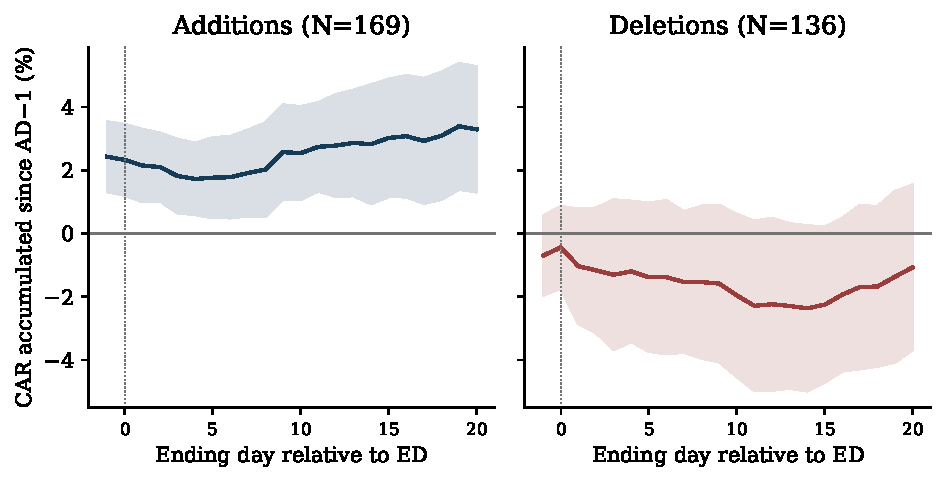
\includegraphics[width=.96\linewidth]{figures/fixed_cohort_path.pdf}
\caption{Cumulative performance through twenty days after implementation. The cohort is fixed separately for additions and deletions in 2017--2026. At every point, the cumulative return starts at AD-1; the horizontal axis gives its ending day relative to ED. The first plotted point is therefore the return already accumulated through ED-1, not a zero normalization. Shading gives pointwise 95\% analytical intervals clustered by review, not a simultaneous confidence band. Counts are 169 additions and 136 deletions.}\label{fig:path}
\end{figure}

\begin{table}[!htbp]
\centering
\caption{Returns before and after implementation on a fixed cohort}\label{tab:horizon_main}
\small
\setlength{\tabcolsep}{5pt}
\begin{tabular}{llrrrrl}
\toprule
Type & Period & Events & Before & After & Cumulative & 95\% interval \\
\midrule
Addition & 2017--2026 & 169 & 2.43 & 0.87 & 3.30 & [1.31, 5.28] \\
Addition & 2022--2026 & 87 & 1.77 & -0.06 & 1.71 & [0.72, 2.69] \\
Deletion & 2017--2026 & 136 & -0.70 & -0.38 & -1.07 & [-3.68, 1.54] \\
Deletion & 2022--2026 & 75 & -0.93 & -0.95 & -1.88 & [-5.72, 1.96] \\
\bottomrule
\end{tabular}
\begin{minipage}{\linewidth}\footnotesize\vspace{5pt}
Returns in percent. Before is AD-1 through ED-1; After is ED through ED+20; Cumulative is AD-1 through ED+20. Each row uses the same events throughout. Intervals are analytical CR1 with review clustering for the cumulative mean. Separate wild-bootstrap tests and post-result exclusions are in the appendix. The horizon is finite and the analysis exploratory.
\end{minipage}
\end{table}


For later-decade additions, the pre-implementation mean is 2.43\% and the subsequent component is 0.87\%, giving 3.30\% cumulatively. The cumulative analytical interval is [1.31\%, 5.28\%]. The after-implementation component's interval is [-0.78\%, 2.51\%], so the result does not establish a separately positive drift after the index change. It shows that the measured cumulative average has not returned to zero by the selected horizon.

The latest block illustrates why a longer horizon must not be selected simply because it produces a smaller $p$-value. Its cumulative estimate is 1.71\%, with an interval of [0.72\%, 2.69\%], but falls to 1.25\% without Sivers and 1.21\% without MSCI overlaps; both latter intervals include zero. The pooled later-decade cumulative mean remains positive in those separate checks. The exclusions were examined after the extension's results were observed. All are reported as exploratory sensitivities, not independent confirmations.

Deletion cumulative returns are less precisely resolved: -1.07\% in 2017--2026 and -1.88\% in the latest block, with both intervals spanning zero. Neither side of the exercise establishes permanent price impact. Twenty trading days remain a finite horizon, and selection, subsequent news and benchmark error can affect cumulative performance throughout it.

\subsection{A comparison within the same firm}

Swedish firms with multiple listed share classes offer an additional comparison. Both classes are exposed to much of the same firm information, while only one may be involved in the index event. If class-specific demand is important, their relative performance is informative. This design improves on a comparison with an unrelated firm in one respect, but it does not make the other class untreated: substitution, arbitrage and shared investor attention can transmit the event to it.

\begin{table}[!htbp]
\centering
\caption{The indexed and sister share classes on the same events}\label{tab:twins}
\small
\setlength{\tabcolsep}{5pt}
\begin{tabular}{lrrrrr}
\toprule
Events & Count & Firms & Index class & Sister class & Difference \\
\midrule
Addition & 19 & 10 & 2.13 & 2.48 & -0.34 \\
Deletion & 20 & 11 & 4.17 & 3.20 & 0.97 \\
Combined & 39 & 13 & 3.18 & 2.85 & 0.33 \\
\bottomrule
\end{tabular}
\begin{minipage}{\linewidth}\footnotesize\vspace{5pt}
Sign-adjusted log market-excess returns in percent for AD-1 through ED+1. Deletion signs are reversed. Each difference subtracts the sister-class mean from the index-class mean on identical events. The combined sample contains 39 events from 13 distinct firms; firm counts by event type overlap. The combined relative-return placebo $p$-value is 0.407. These selected log-return observations cannot be subtracted from the main arithmetic-CAR sample to identify a causal component.
\end{minipage}
\end{table}


Table~\ref{tab:twins} reports both legs of the comparison on identical events. Across 39 events from 13 firms, the sign-adjusted log market-excess return is 3.18\% for the index class and 2.85\% for the sister class, leaving a relative return of 0.33 percentage points. The event-weighted placebo $p$-value for the relative return is 0.407. For the 19 additions alone, the corresponding means are 2.13\% and 2.48\%, giving a relative return of -0.34 points. These observations are a selected subset of the full sample and use log relative returns, so they cannot be subtracted from the 2.15\% main estimate as a causal decomposition.

The small relative estimate does not establish that index demand has no effect. Some of the difference may be transmitted to the sister class; some firms occur repeatedly; and thin trading or changes in return sources affect the measurement. A source-consistent subset contains 29 events from nine firms and has a relative mean near 0.04 points. The placebo construction does not jointly preserve all firm and review dependence. This extension therefore indicates that the available within-firm sample does not precisely isolate a class-specific response, while keeping both stock legs visible rather than treating the comparison as an unexplained null.

A separate size-screened comparison provides a complementary check. After removing the one-day overlap between its pre-return control and outcome, the later addition coefficient is 1.65 percentage points, with a 95\% analytical interval of [0.48, 2.83]. Restricting comparisons to the main market gives 1.49 points, with an interval of [0.24, 2.74]. The correction preserves the sample and other controls. These remain conditional differences rather than threshold-based causal estimates; Appendix~\ref{app:comparisons} reports the full before-and-after results.

\subsection{Limits and implications}

The main unresolved identification issue is that index membership is related to firm characteristics and prior performance. Market adjustment, composition controls and comparison securities do not remove every reason that selected stocks may have different returns. The study consequently establishes associations around observed changes rather than the causal effect of assigning a stock to OMXSB.

Measurement is a second constraint. Some historical notices still require field-by-field reconciliation; return availability excludes part of the source inventory; and absent holdings rows do not independently prove zero positions. The shares-outstanding denominator is available in the vendor panel on ED for every retained complete holdings event, but that does not establish the freshness of the underlying issuer filing. The adjustment screen reduces early coverage particularly heavily. These issues matter most for long-run demand comparisons and are recorded in Appendix~\ref{app:holdings}.

Statistical precision is a third constraint. Many securities share the same review, the latest period has only nine review clusters, and the full research record contains multiple outcomes and specifications. The uncertainty checks prevent a point estimate from being treated as more informative than it is; they are not a separate economic explanation for the result. Some sparse auxiliary bootstrap intervals also vary across numerical environments. The main conclusions do not rely on those unstable endpoints.

For investors, the evidence describes the timing and magnitude of observed returns; it is not a tested net trading strategy. The estimates do not deduct transaction costs, impose realistic execution rules or guarantee that membership changes were predictable. For research on indexing, the central implication is narrower: full-window returns, immediate announcement responses and implementation trading should be distinguished when the event calendar changes. In this sample, the case for a completely vanished Swedish addition association is weak, while the case for a precisely identified historical elasticity decline is weaker still.
\FloatBarrier
